\section{Necessity of in-kernel NF chaining}
The original Internet protocol suite TCP/IP was standardized in the 1970s and the TCP/IP stack was first implemented in BSD OS in the early 1980s. Since then lots of efforts were made to implement this protocol in other platform like Linux. At first mutual communication via the Internet was only leveraged in military and commercial use. But as the Internet grew bigger and network application such as file sharing among distant entities gained popularity, the networking function by TCP/IP became a “commodity service”. This means that the availability of this protocol is demanded by the majority of normal users and therefore it became an essential component in the kernel. 

 38 years after the first implementation of network stack in kernel (BSD), demands against networking function has also progressed. Kernel now supports not only TCP/IP but also lot of other protocols and simple per packet network function such as Firewall or NAT. They are implemented by Netfilter system in linux. One of the recent trend in network industry is, as mentioned, Network Function Chaining and this is realized either by traditional proprietary hardware or virtualization technology. We believe that this NF chaining should be implemented in the kernel of general purpose OS, likewise network stack was integrated in kernel decades ago. Even though there are certain number of advanced NFs that are required by network nodes and certain users, the only way to run them (except buying expensive dedicated hardware) is with the help of high cost virtualisation technology. That is why we propose NF chaining mechanism in the kernel. Its aims is to realize the chaining of NFs that are not executable by the existing Netfilter system in the Linux. 
 
 However we do not think that all kinds of advanced NFs can work within the kernel space. In section 3.1.1 and 3.1.2, functions that organize NFs are categorized and example of executable and non-executable NFs are listed. And in chapter 3.2, the contribution of kernel-based NFCI node in Wide Area Network (WAN) is described. 
 
 \subsection{Categorization of Network Functions}
 Functions in NFs are categorized into two types:
 \begin{itemize}
 	\item Simple functions: NFs often include functions like read/write of the packet header or read of application payload. The former process is already realized by Netfilter for NF such as NAT. The latter process is for example used to inspect the content of the message (application payload). The mean of inspection determines whether it is feasible in the kernel or not. If it is a  process such as hashing the payload to compare with a value or understanding the application-specific protocol, it is categorized in this simple functions. The detail of the NFs that have such functions are described in the chapter 3.2. 
 	\item Complicated functions: When addressing application payload in NF, dedicated libraries are sometimes used for sophisticated service. This often requires lot of calculation and it is not suitable to place such function in the kernel. It is because if the process gains the highest priority, it will most likely takes up all the CPU according to the Complete Fair Scheduling (CFS) in Linux. Therefore they should be virtualized and put in the user space to guarantee the isolation of resource like CPU. 
 \end{itemize}
 Simple functions described above are regarded executable in kernel space. 

\subsection{Example of Network Functions and its realizability in kernel}
NFs are roughly divided into the following two categories. One is kind of NFs that need to work on the requesting node to provide the service, being security related functions like firewall. In the point that security measures that are more sophisticated than simple firewall will be essential for the majority of users, this kind of NFs are defined as commodity service in this paper. And another kind is NFs that are to be placed on network nodes to provide better performance in overall network, such as Traffic Engineering (TE). 
\begin{itemize}
	\item Network Functions of Commodity Service\\
		Although NFs such as Firewall and NAPT which can check up to transport layer (Layer 4) are already implemented in kernel, NFs that require information that resides higher than Layer 4 are not. As example of latter NFs, there are Web Application Firewall (WAF) and Application Layer Gateway (ALG). 
		\begin{itemize}
			\item WAF\\
				WAF is a security control to protect web applications against attacks that traditional firewall could not prevent, such as SQL injection and cross-site scripting. WAF detects the threats by examining incoming HTTP traffic. Specifically, it analyzes all HTTP requests (GET and POST requests) to apply defined rules to identify malicious traffic. Set of signatures that represents patterns that are components of well known attacks are used against traffic payload. A pattern match of signature and the traffic payload means that it's illegal traffic.
			\item ALG\\
				ALG is a firewall for specific application protocols such as SIP (Session Initiation Protocol) and FTP (File Transfer Protocol). ALS acts an intermediary between the client and application server and controls whether to allow or deny traffic to application server. It recognizes application specific commands in application payload and offers security controls over them. 
		\end{itemize}
	
		In the case of WAF, pattern matching of signature is what is basically done. Pattern matching can be checked against the whole payload of a packet or only the first few tens of kilobytes of the payload. The first case may require specific libraries and complex calculation and thus is not pragmatic to implement in kernel. But in the second case, only the first part of the payload will be hashed and this value is checked against the signature. Comparison of a hashed value is a simple process that also kernel module of OVS conducts when searching the flowtable. So the latter is feasible to implement in kernel and therefore is subject to our NF. 
		
		In the case of ALG, it is necessary to understand the application-specific protocol in layer 5. For example in FTP, a command "GET" can be placed in application payload to get file from the server. To recognize the complete message of the application, it is necessary to see the whole payload. For example in case of TCP/IP, the IP stack that get data from transport stack will chop off the data to be sent up to the Maximum Segment Size (MSS), put them in TCP segments and then encapsulate them in IP packets. In order to get the original payload before it was divided by MSS, TCP segments need to be reassembled. Since Netfiler only supports NFs that process per packet, it is yet not realized in kernel. Reassembling packets to realized NF such as ALG is our future work.
		
	\item Network Functions of TE\\
		TE is a method of optimizing the performance of carrier network by dynamically analyzing and regulating the behavior of the data transmitted over the network. Representative NFs of TE is Multipath Routing and Network Caching. 
		\begin{itemize}
			\item Multipath Routing\\
				Mulitpath Routing supports multiple paths for a transmission of streams of data between two end points. This provides better utilization of available bandwidth, higher fault tolerance and load balancing over available resources. The process works as follows: All available paths to the destination is aggregated into a single virtual path. Packets from the applications are gathered to this virtual path and they are distributed to the actual physical path via mechanism such as round-robin or weighted fair queuing. By offering packets to all paths, available bandwidth can be fully utilized and even in the case of link failure streams can reach the endpoint continually.  
			\item Network Caching\\
				Large percentage of web traffic consists of much of the same requests to web servers. These identical traffic can be significantly reduced by network caching technology. It keeps frequently accessed web content in a cache storage close to the requesters. The process works as follows: A user accesses a web page. If the local cache storage has the cache of the requested content it will be transferred to the user without the trouble of accessing the web server. Otherwise the local network cache get the content from the web server to store in the storage so that the next requester can use the cached content. 
		\end{itemize}
		These TE functions are also targeted NFs in the kernel-based NFV in the future. 
\end{itemize}

\section{The role of Kernel-based NFCI node in WAN}
\subsection{The structure of WAN and the position of Kernel-based NFCI node}
In WAN, there are companies as Network Service Provider (NSP) and Internet Service Provdier (ISP). NSP owns networking hardwares such as routers and switches (network node) that build up network infrastructure and sells network resources as bandwidth to ISP. And ISP provides the network resources to users. Our future vision is that hardware routers or switches will be replaced by general purpose OS, and in that case kernel-based NFCI plays the roles of network node as well as normal user node. This means that basic NF chaining would be executed on each of network or user node by Kernel-based NFI without deploying virtualization technology. 

\subsection{Placement of Network Function}
Depending on the kind of the NF, the place where the NF should be loaded is determined. For instance security related NF such as firewall, WAF should run in the requesting user node. On the other hand, TE related NFs, load balancer, and so on are placed by NSP on network nodes. In both cases, a NF that is sent from the NSP are source code of kernel modules that makes up the NF. The kernel modules will be then compiled in the environment of the installed node and start to function. 
Figure \ref{fig: overview_1} and figure \ref{fig: overview_2} show the placement of the two kinds of NFs in WAN. In addition to ISP and NSP, there are network nodes and user nodes which are all OS of kernel-based NFV. 

\begin{figure}[htbp]
	\begin{minipage}{0.5\hsize}
		\begin{center}
			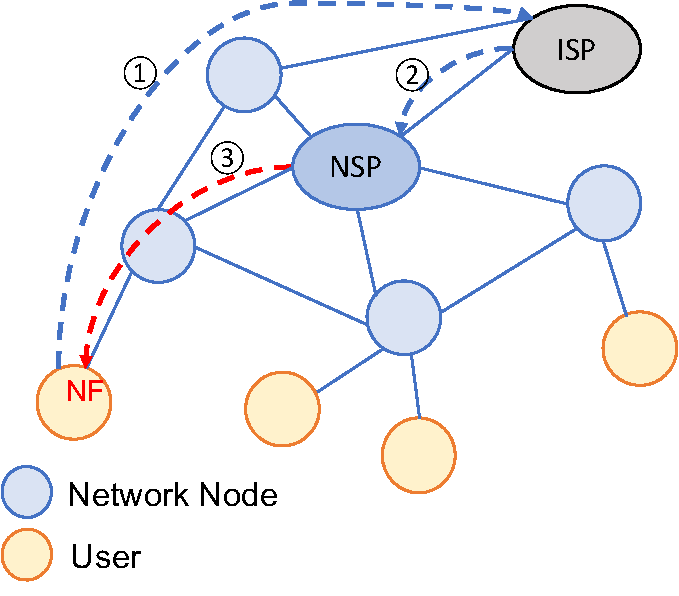
\includegraphics[width=75mm]{pics/overview_1.pdf}
		\end{center}
		\caption{NF request by user}
		\label{fig: overview_1}
	\end{minipage}	
	\begin{minipage}{0.5\hsize}
		\begin{center}
			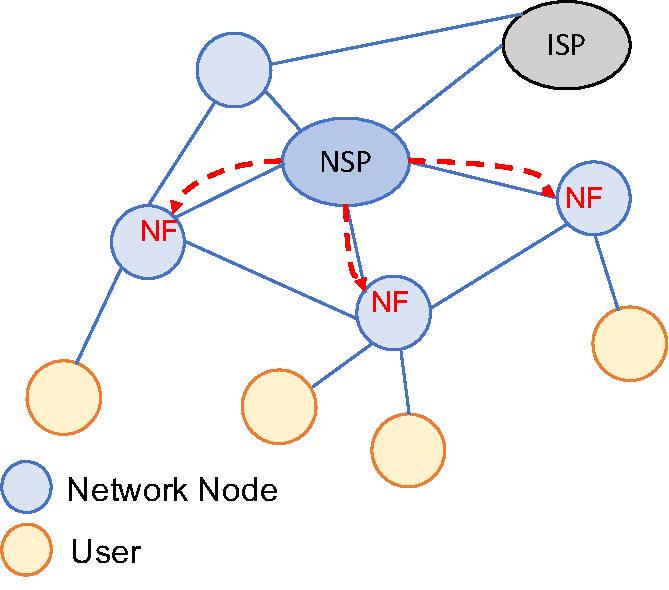
\includegraphics[width=75mm]{pics/overview_2.pdf}
		\end{center}
		\caption{NF placement by NSP}
		\label{fig: overview_2}
	\end{minipage}	
\end{figure}

\ref{fig: overview_1} explains process where the former NFs are loaded. 1) User node requests a NF to ISP. 2) ISP then tells the NSP where to load the requested NF, in this case in the requesting user node. 3) NSP loads the NF in the right node. 

\ref{fig: overview_2} depicts the case of latter NFs placement. These NFs are not requested by user nodes but the NSP itself loads them in network nodes. This is because latter NFs such as TE related ones contribute to the overall higher performance in networking such as better utilization of bandwidth and hence producing more profit for the company. When the NSP decides that the traffic between user A and user B should pass through a NFs of this kind, there are two ways to realize this. The first way is to load necessary NFs in network nodes on the shortest path between users. The second way is to user Network Service Header (NSH) to change the path of the traffic to traverse network nodes that already installed NFs in demand. 


	\begin{itemize}
		\item Loading on shortest path\\
			The former way is easier to do in terms of no need of modifying the path. But it is not hard to imagine that this will leads to redundant placement of NFs in network nodes. As each time a new traffic flow has to be processed by NFs, it is likely that the same NFs will be placed in different network nodes. 
		\item NSH\\
			NSH is added in each packet header as an information of designated service function path in a single administrative domain. NSH describes a sequence of service function nodes that the packet must be routed prior to reaching the destination. NSH is inserted between the original packet and outer network encapsulation such as MPLS, VXLAN, etc. Important information is placed in service path header in NSH. It consists of 24 bits of Service Path Identifier (SPI) and 8 bits of Service Index (SI). SPI identifies service function path and SI is an indication of number of processed Service Function. 
			
			Network Function chaining by NSH requires the following three components, control plane, Service Classifier (SC) and Service Function Forwarder (SFF). As in the figure \ref{fig: NSH} , there is ingress and egress routers in the network marked with SC and network nodes with SFF and SF. Control Plane is in charge of creating service chain and setting the regarding information in SCs and SFFs. 
			
			As a packet enters ingress router, SC classifies the packet according to the pre-defined policy and apply NSH to the packet with appropriate SPI and SI value. And the packet is sent to the next hop to be processed by FSS. FSS determines the forwarding destination for the first SF based on the NSH and insert overlay header (e.g., VXLAN header) for transmission. When the packet arrives at the SF, the overlay header is striped and the SF takes action. Subsequently SI value is decremented by one and FSS applies new NSH and overlay header to transmit to the next SF. When the service function chaining completes, NSH will be removed at egress SC and normal forwarding resumes.   
			
			The advantage of NSH in comparison with OpenFlow-based network operation is the scalability. To use OpenFlow for programming NF chaining, it is necessary to set up all the nodes in the network with OVS. OpenFlow uses Match-Action flowtable which directs packets regardless of the shortest path. If there is a node that does not understand OpenFlow in the same network it could cause loop in the network. So OpenFlow can be used in a single datacenter network or interconnection between small-scaled datacenters in the biggest use case. On the other hand, NSH does not require all the nodes to be NSH-aware. Only the nodes that host Service Functions and ingress/egress routers should understand NSH protocol. This is because the routing from a FSS to the next FSS is done by overlay network so that non-NSH-aware nodes between them can route the packet with shortest path policy. When using NSH, configuring NF chaining in large scale network between datacenters is also possible. From those reasons, NSH is the technology that we want to use for Kernel-based NFV in the future. 
	\end{itemize}
	
\begin{figure*}[t]
	\centering
	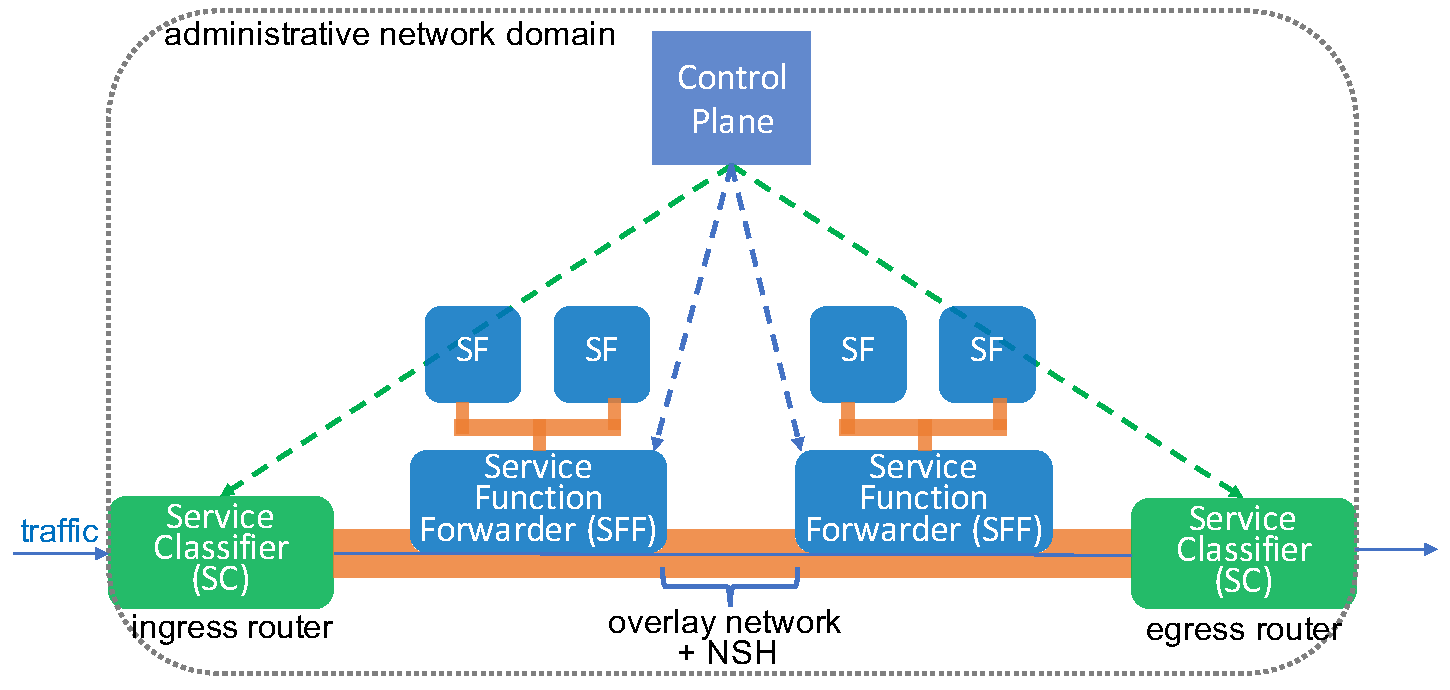
\includegraphics[width=120mm]{pics/NSH.pdf}
	\caption{NSH Architecture}
	\label{fig: NSH}
\end{figure*}

\subsection{Scope of the paper}
This paper focuses on the data plane of NF chaining rather than control plane.  Specifically, NF chaining mechanism for per packet process in a single host is implemented. The system of reassembling IP packets to acquire the original payload for NF such ALG remains as future work. 










